% -*- coding: UTF-8 -*-
% hello.tex

\documentclass[UTF8]{book}

\usepackage{xeCJK}
\usepackage[utf8]{inputenc}

% load paralist before enumitem
\usepackage{paralist}

\usepackage{hyperref}
\hypersetup{pdftex,colorlinks=true,allcolors=blue}
\usepackage{hypcap}

\usepackage{color}
\usepackage[usenames, dvipsnames, svgnames, table]{xcolor}
% \pagecolor{gray}

\usepackage{makeidx}
\makeindex

\usepackage{amsmath}
\usepackage{mathtools}

\usepackage{listings}
\usepackage{multicol}
\usepackage{fancybox}
\usepackage{tcolorbox}
\usepackage{enumitem}

\usepackage{indentfirst}

% table
\setlength{\arrayrulewidth}{1pt}
\setlength{\tabcolsep}{16pt}
\renewcommand{\arraystretch}{2.5}
\newcolumntype{s}{>{\columncolor[HTML]{AAACED}} p{3cm}}

\arrayrulecolor[HTML]{DB5800}

\usepackage{tikz,mathpazo}
\usetikzlibrary{shapes, arrows, chains, trees, arrows.meta}

% \bibliographystyle{plain}
% \bibliography{math}

\tikzset{%
  >={Latex[width=2mm,length=2mm]},
  % Specifications for style of nodes:
            base/.style = {rectangle, rounded corners, draw=black,
                           minimum width=4cm, minimum height=1cm,
                           text centered, font=\sffamily},
  activityStarts/.style = {base, fill=blue!30},
       startstop/.style = {base, fill=red!30},
    activityRuns/.style = {base, fill=green!30},
         process/.style = {base, minimum width=2.5cm, fill=orange!15,
                           font=\ttfamily},
}

% 摘录
\usepackage{verbatim}
\usepackage{libertine}
\usepackage{graphicx}
\usepackage{framed}

\newcommand*\openquote{\makebox(25,-22){\scalebox{5}{``}}}
\newcommand*\closequote{\makebox(25,-22){\scalebox{5}{''}}}
\colorlet{shadecolor}{Azure}

\makeatletter
\newif\if@right
\def\shadequote{\@righttrue\shadequote@i}
\def\shadequote@i{\begin{snugshade}\begin{quote}\openquote}
\def\endshadequote{%
\if@right\hfill\fi\closequote\end{quote}\end{snugshade}}
\@namedef{shadequote*}{\@rightfalse\shadequote@i}
\@namedef{endshadequote*}{\endshadequote}
\makeatother

\usepackage[normalem]{ulem}
\usepackage{soul}

\newcommand{\hlc}[2][yellow]{{%
    \colorlet{foo}{#1}%
    \sethlcolor{foo}\hl{#2}}%
}

% todonode
\usepackage{lipsum}                     % Dummytext
\usepackage{xargs}                      % Use more than one optional parameter in a new commands
% 
\usepackage[colorinlistoftodos,prependcaption,textsize=tiny]{todonotes}
\newcommandx{\unsure}[2][1=]{\todo[linecolor=red,backgroundcolor=red!25,bordercolor=red,#1]{#2}}
\newcommandx{\change}[2][1=]{\todo[linecolor=blue,backgroundcolor=blue!25,bordercolor=blue,#1]{#2}}
\newcommandx{\info}[2][1=]{\todo[linecolor=OliveGreen,backgroundcolor=OliveGreen!25,bordercolor=OliveGreen,#1]{#2}}
\newcommandx{\improvement}[2][1=]{\todo[linecolor=Plum,backgroundcolor=Plum!25,bordercolor=Plum,#1]{#2}}
\newcommandx{\thiswillnotshow}[2][1=]{\todo[disable,#1]{#2}}
%

\usepackage[simplified]{pgf-umlcd}

\title{LICH架构文档}
\author{董冠军}
\date{\today}

\begin{document}

\maketitle
\tableofcontents

\listoftodos[Notes]

\part{项目管理}

\chapter{移动集采}

产品评估:功能和质量。质量包括:可靠性,性能,QoS,可扩展性(负载均衡),用户体验(管控,交互,接口)等方面。

性能不是一个值,而是不同场景下的特征曲线。性能是系统配置和负载的函数:$P=F(S, W)$。
精简配置,快照,故障,实现机制等因素都会影响性能及其抖动。

\section{CheckList}

对标\hl{移动集采测试规范}

\subsection{Hardware}

同质化项:
\begin{enumbox}
\item 开机Logo
\item 贴标
\item 开机卡,需断电源
\end{enumbox}

\subsection{Software}

标前测试:
\begin{enumbox}
\item 管理系统相关Logo
\item 上架
\item 安装
\item 性能测试
\end{enumbox}

BUG
\begin{enumbox}
\item etcd依赖于物理时间
\item bcache拔cache盘后需要重启服务器
\end{enumbox}

性能:
\begin{enumbox}
\item \hl{打开chunk parallel开关}
\item \hl{禁用core}
\item 优化Log
\item O3编译
\item -g
\item 代码段
\end{enumbox}

功能:
\begin{enumbox}
\item IPv6
\item SNMP
\item bcache
\item Recovery
\item Balance
\item QoS
\item QoS 1.1抖动幅度是否需要可配置
\end{enumbox}

\section{LEFT}

\subsection{可靠性}

诊断写错误效率太低,需要完善分析方法和工具。

log分析法

chunk,副本级数据一致性校验(disk bitmap和sqlite)。

disk bitmap无,而sqlite有。会导致什么结果?多个sqlite记录指向同一个磁盘位置。

\subsection{性能}

clock(副本一致性)

msqqueue(操作日志)

卷分为chunk,chunk有多副本。在独立的部分之间,尽量并发。

多个卷,要注意session和controller平衡。

在分配阶段,一个chunk的持久化信息,包括三部分:diskmd,sqlite和table2 meta。

并发,锁的粒度。

\subsection{删除}

删除卷,比删除快照更早完成,导致快照无法删除

回收replica时,sqlite有,disk bitmap无。

并发删除一个卷的多个快照会如何?

有节点不在线,无法完成删卷操作,反复重试而无果。

timer不工作,是堵塞还是其它?

删除队列里的快照,也计入快照数,满足一下不等式:root+auto+rmsnap+user <= 256。

提供强制回收的工具

\subsection{平衡}

批量分配卷

\subsection{md5sum}

每个chunk有几种状态:没分配,分配,分配并填0。
第一种和第三种状态等价,第二种状态结果不可知。

\section{TODO}

\begin{enumbox}
\item Pool
\item Volume size
\item Volume mv and copy
\item Volume IOPS QOS
\item Mapping
%\item Recovery
%\item 可靠性 Robustness
%\item Load Balance
%\item Performance
\item extentability
\end{enumbox}

\section{重要问题}

\subsection{存储池}

模型:概念及其关系。

重建状态和速度按存储池进行统计。

\subsection{卷}

\begin{enumbox}
\item 精简配置
\item 三副本
\item 扩容
\item 卷的QoS:IOPS
\item 全量拷贝和增量拷贝
\end{enumbox}

三副本 \info{三副本性能}

\subsection{快照}

\begin{enumbox}
\item 显示卷和快照的创建时间,名称,宿主,\hl{容量,存储池}。
\item 快照树是必须的
\item 快照验证:每个快照关联一个数据集。
\end{enumbox}

\subsection{映射}

数据访问和隔离机制,应按\hl{最小权限原则设计}。主机仅能访问映射到该主机的卷

\subsection{故障处理}

\begin{enumbox}
\item IO抖动
\item 重建
\end{enumbox}

\subsection{数据恢复}

触发策略,QoS,性能,状态。

\begin{enumbox}
\item 在线调整策略:应用优先,或恢复优先。
\item 负载调整到原来的20\%时,数据重建效率。
\item 显示恢复速度和状态,区分实际重构的,和跳过的
\item 拔出硬盘的存储池降级(数据冗余度发生下降,目前恢复进程是节点级的,与存储池没有直接关系,并且,在节点的维度上,存储池是有覆盖的,overlay network,\hl{按卷进行汇总})
\item 磁盘漫游,存储系统不发生重建,且数据无异常
\item 模拟故障:单磁盘,单节点,单机架。要求:无读写中断。
\end{enumbox}

要研究的问题:
\begin{enumbox}
\item 在业务负载限定为标准负载的20\%的情况下,恢复性能如何?
\item 如业务IO和数据恢复并存,数据恢复会挤压到很小。原因是什么?\hl{如何做到恢复优先}?
\item 拔盘后,感知状态变化较慢。如\verb|md_chunk_set|不持久化meta,有无副作用?恢复时,也可不持久化。
\end{enumbox}

\subsection{负载均衡}

均衡有数据均衡和负载均衡之分。

单卷的负载均衡,因为FusionStor卷控制器绑定到core上,只能利用单核能力。
CPU利用率上有瓶颈。同时,开启polling模式,会独占core cpu。

\subsection{QoS算法}

卷的IOPS和带宽,数据恢复的QoS,采用同一算法:令牌桶Token bucket。

按恒定速度往桶里加入令牌,任务会消费令牌。如果令牌不足,则任务进入等待状态。
目前,等待时间采用polling策略。等待一个较小的值(200us),唤醒后重新检查。

接口保持不变。

\begin{tcolorbox}
fio队列深度过大,iscsi会有优化,进行IO聚合提交。这样一来,前端工具看到的IOPS可能会有所不同。
但是,各层观察到的带宽应该一致,保证流量守恒。
\end{tcolorbox}

\subsection{Cache}

BCache

\subsection{Misc}

VAAI

\section{不需要做的项}

\begin{enumbox}
\item 一致性组
\item 同步/异步远程复制
\item EC
\end{enumbox}

\chapter{任务清单}

%\pagestyle{empty}
\todo[inline]{The original todo note withouth changed colours.\newline Here's another line.}
\lipsum[11]\unsure{Is this correct?}\unsure{I'm unsure about also!}
\lipsum[11]\change{Change this!}
\lipsum[11]\info{This can help me in chapter seven!}
\lipsum[11]\improvement{This really needs to be improved!\newline\newline What was I thinking?!}
\lipsum[11]
\thiswillnotshow{This is hidden since option `disable' is chosen!}
\improvement[inline]{The following section needs to be rewritten!}
\lipsum[11]
%\newpage

\section{原生卷}

\begin{tcolorbox}
\begin{compactenum}
    \item 存储池
    \item 数据恢复性能
    \item \sout{async sqlite}
    \item \hlc{batch sqlite}
    \item Allocate的性能
    \item 精简配置,快照对性能的影响
    \item 快照树
    \item 单卷快照的数量
    \item SSD Cache
    \item Redis Cache
    \item 异步远程复制
    \item VAAI
    \item FC (+VAAI)
\end{compactenum}
\end{tcolorbox}

\section{关键特性和过程}

\begin{compactenum}
    \item flush, load and recovery
    \item 保护模式 safe mode
    \item 存储分层
    \item 命令行工具,扩展卷和快照相关操作到LSV
\end{compactenum}

\section{兼容性}

\begin{compactenum}
    \item 版本演进
\end{compactenum}

\section{Pool}

\begin{compactenum}
    \item Resource Pool
\end{compactenum}

\section{Volume}

\begin{compactenum}
    \item new format: row2
    \item new format: lsv
    \item vol max size 256T+
    \item vol resize?
    \item all zero's chunk
\end{compactenum}

\section{快照}

\begin{compactenum}
    \item 支持60000+快照
    \item consistency group
    \item 每个snap的大小等信息
    \item snap大小对GC策略的影响
\end{compactenum}

\section{一致性/正确性}

\begin{tcolorbox}
\begin{compactenum}
    \item 底层数据检验工具(chunk0, volume, log/gc, bitmap, wal, rcache)
    \item 内置质量,各模块添加自校验机制,方便诊断数据正确性问题(assert + log + test)
    \item 加强断言:pre和post条件,变量变化规则,不变式,基本假设等
    \item 日志用tag/keywork和timeline,以便于跟踪一个对象的变化历史,用一个或多个维度贯穿起来,用于辅助诊断
    \item 增加CHUNK\_HISTORY,以时间线方式,跟踪记录CHUNK变化的生命周期
\end{compactenum}
\end{tcolorbox}

\section{性能}

性能是负载和资源的函数, $P=F(W, R)$。

\begin{tcolorbox}
\begin{compactenum}
    \item 创建卷时,rcache分配了4096M的SSD cache,可以延迟分配
    \item \textcolor{red}{rcache 顺序IO随机化问题}
    \item wbuf 顺序IO随机化问题
    \item 系统启动时间
    \item 预填充lich chunk
    \item GC策略和算法
    \item 统计基础操作的开销,作为性能分析的基础
\end{compactenum}
\end{tcolorbox}

\section{负载}

\begin{tcolorbox}
\begin{compactenum}
    \item IO队列深度
    \item IO平均大小
    \item IO读写大小
\end{compactenum}
\end{tcolorbox}

\section{资源}

\begin{tcolorbox}
\begin{compactitem}
    \item 内存使用量过大
    \item 内存泄漏
    \item 磁盘利用率不足
    \item 网络带宽:瓶颈或利用率不足
    \item 中断
    \item soft lock up?
\end{compactitem}
\end{tcolorbox}

\section{故障处理}

\begin{compactenum}
    \item \change{故障域,不能中断IO}
    \item 节点间负载均衡(<20\%)
\end{compactenum}

\section{Misc}

\begin{tcolorbox}
\begin{compactitem}
    \item FC
    \item Remote copy
    \item SSD cache
    \item EC
    \item 有效容量的比例
    \item 热插拔
    \item 磁盘漫游
    \item 在线扩容
    \item 滚动升级
\end{compactitem}
\end{tcolorbox}

\section{DONE}

\begin{compactenum}
    \item VAAI [+xcopy]
\end{compactenum}


\part{FusionStor}

\chapter{模型}

\begin{tikzpicture}[show background grid]
    \begin{class}{Disk}{6, 0}
    \end{class}
    \begin{class}{Pool}{6, 2}
    \end{class}
    \begin{class}{Volume}{6, 4}
    \end{class}
    \begin{class}{Host}{6, 6}
    \end{class}
    \begin{class}{Cluster}{0, 2}
    \end{class}
    \begin{class}{Snapshot}{0, 4}
    \end{class}

    \composition{Cluster}{pools}{1..*}{Pool}
    \composition{Pool}{disks}{1..*}{Disk}
    \composition{Pool}{volumes}{1..*}{Volume}
    \composition{Volume}{mapping}{*..*}{Host}
    \composition{Volume}{snapshots}{1..*}{Snapshot}
\end{tikzpicture}

\section{Cluster}

整体

\section{Pool}

把物理节点划分为不同的保护域,一个卷的所有数据只出现在一个保护域内。卷可以跨保护域进行复制和迁移。

默认一个,包括所有节点。

% 保护域是物理节点的划分,存储池是存储介质的划分。每块盘只能出现在一个存储池里。

Pool: 逻辑容器

故障域有粒度之分,如磁盘,节点,机架,机柜,数据中心。

存储池内,要满足故障域规则:一个chunk的不同副本,分布在不同的故障域内。\label{rule:faultset}

在初次分配,再平衡和恢复等过程中,都需遵循这些规则。

\begin{tcolorbox}

可以参考ceph的CRUSH实现。bucket和device定义了集群的物理拓扑结构,rule定义了数据存取规则,
pool上关联rule,从而定义了pool中卷数据的放置规则。设备即OSD,对应一个物理磁盘。

***

存储池可以取代保护域,定义所有对象的存放位置是一个节点集。

***

存储池可以用来实现tier cache。重定向IO到cache pool。

***

统一概念:保护域,故障域,存储池,pool。Consistency Group不同于pool,与物理存取无关,
而是卷的逻辑集合,卷可以来自不同的pool。

\end{tcolorbox}

与存储池有什么同和异?存储池可以看做关联了磁盘的pool,可以看做pool的子类。

属性:
\begin{enumbox}
\item 配额
\item 复制类型:副本 OR EC
\item 磁盘列表
\item 定义精简池
\item 存储池上可以指定卷的副本数
\item \hl{有足够的故障域,且不同故障域配置一致的资源量}
\end{enumbox}

操作:
\begin{enumbox}
\item 创建
\item 删除
\item 扩展(添加磁盘到\hl{已存在的存储池},该映射关系持久化到本地,同步到admin节点)
\item 缩容(从存储池中移除磁盘,引发数据重建过程)
\item \hl{自动或手动按磁盘速率进行存储池分级划分}
\item 不同存储池之间,卷的复制
\item 不同存储池之间,卷的迁移,可在线或离线
\item 存储池级别的统计信息
\end{enumbox}

% 存储池是disk的集合,与节点无关。但disk所在的节点构成存储池的节点列表,不同存储池的节点可能覆盖。

存储池下,可以创建volume。没有关联磁盘的存储池,不能创建卷。

\hl{chunkid到磁盘物理位置有两级映射:chunk的副本节点列表,节点内chunkid到物理地址的映射}。

在为卷分配chunk的时候,需要确定各个副本的物理存储位置。当前实现是返回不同副本的节点列表。
如果指定了存储池,就需要在存储池所在的节点范围内进行分配。同时要满足故障域和数据均衡规则。

\begin{tcolorbox}
移动采集中存储池要求,相比于目前的逻辑pool,更多是一种设计上的退步。
存储虚拟化的目标,是物理位置无关。我们可以基于逻辑容器,实现基于策略的管理。
所以,\hl{从实现层面,要保留当前pool的功能,按照系统配置确定pool的类型}。
\end{tcolorbox}

% 存储池内,要满足故障域规则(\ref{rule:faultset})

步骤:
\begin{enumbox}
\item 创建pool,但此时不能创建pool的元数据chunk,因为还没有绑定磁盘(需要一全局的地方,存储pool名字)
\item 添加磁盘到pool,通知admin节点
\item 当在pool下面创建卷的时候,前提条件是已准备好磁盘,生成pool元数据chunk(位于同一pool里)。
\end{enumbox}

pool元数据chunk必须位于自己的存储池内,如果分布在不同的存储池,不满足故障域条件。

pool引导信息可以存在rootable里。

\section{Volume}

属性:

操作:
\begin{compactenum}
    \item rename
    \item resize \info{在线扩容}
    \item mv
    \item copy \change{全量拷贝/增量拷贝} \change{跨存储池拷贝} % change不能出现在box里
\end{compactenum}

\section{Snapshot}

snapshot隶属于卷,无卷则无快照,快照组织成快照树,其中有且只有一个快照是可写快照,即卷的写入点。

\section{Mapping}

数据隔离/ACL,数据保护

卷对主机的可见性。一个卷只有映射给了某主机,才可以被该主机访问。


\section{Consistency Group}

一致性卷组

\begin{shadequote}
Consistency Groups could be useful for Data Protection (snapshots, backups) and
Remote Replication (Mirroring).

The Mirroring support will allow to setup mirroring of multiple volumes in the
same consistency group (i.e. attaching multiple RBD images to the same journal
to ensure consistent replay).

There is already an interest to implement this functionality as a part Mirroring feature:
http://tracker.ceph.com/issues/13295

The snapshot support will allow snapshots of multiple volumes in the same
consistency group to be taken at the same point-in-time to ensure data
consistency.
\end{shadequote}

\chapter{硬件架构}

\section{节点}

\subsection{添加节点}

负载均衡,需要重新平衡数据

\subsection{删除节点}

恢复


\section{Pool}

\section{Disk}

\subsection{Tool}

操作磁盘的工具
\begin{enumbox}
\item hdparm set/get hard disk parameters
\item iostat
\item lsscsi
\item udevadm
\item sg\_inq
\item disk2lid
\end{enumbox}

\subsection{Cache}

Disk Cache

关闭磁盘cache,防止出现数据不一致情况。怎么关闭呢?相关管理工具是什么?

磁盘的设备驱动,linux kernel的块设备IO架构

NVMe具有什么特征?

\subsection{RAID}

Ctrl+R进入bios的RAID控制界面。通过bios进行的管理操作,进入系统后用MegaCli等命令行工具也能完成。
且更为方便。

每个控制器管理一个或多个enclosure,每个enclosure有固定数量的slot。每个slot对应一块物理设备。
每个物理设备处在不同的firm 状态,这些状态可以相互转换。在物理设备之上,构建虚拟设备。

带电池BBU的情况下,可以打开RAID cache。

NVMe在不在RAID里,系统盘呢?看不到系统盘,是因为系统盘不在RAID控制器管理的slot内?

缓存盘做出JBOD,数据盘RAID0

全部是JBOD,性能影响较大。

\subsection{Tier}

检测磁盘分层,支持两个磁盘分层:0和1, 0是SSD,1是HDD。

\subsection{Meta}

磁盘管理元数据目录:/opt/fusionstack/data/disk:
\begin{compactitem}
\item disk
\item \hl{bitmap}
\item info
\item tier
\end{compactitem}

对每块磁盘,开头的1M是引导信息,通过bitmap来进行空间管理。
引导信息包含了所在节点信息,所以只能在节点内进行磁盘漫游。

所在源文件是\emph{diskmd.c}。调用fnotify\_register监控磁盘目录的变化,进而添加或移除相应磁盘。

每个节点最多可以添加256个磁盘。

sqlite3划分为10个db文件,chkid信息hash到相应的db。每个db包含两个table:metadata和raw。

\begin{lstlisting}[frame=single]
CREATE TABLE metadata (key text primary key, 
    disk integer, 
    offset integer, 
    parent text, 
    priority integer, 
    meta_version integer, 
    fingerprint integer, 
    wbdisk integer);

CREATE TABLE raw (key text primary key, 
    disk integer, 
    offset integer, 
    parent text, 
    priority integer, 
    meta_version integer, 
    fingerprint integer, 
    wbdisk integer);
\end{lstlisting}

\subsection{状态机}

拔盘-恢复未完成,如何加入?(符号链接丢失,别的文件处在可用状态,重启lichd,修复符号链接)

拔盘-恢复完成,如何加入?

\section{Advanced}

NVMe

RDMA/DPDK/SPDK

AFA

\chapter{元数据管理}

etcd,存储池,目录,卷,快照,映射

结合lsv,row snapshot考虑当前的元数据管理,看看会有哪些瓶颈?

\section{元数据}

最重要是chkinfo结构体,表示一个chunk的若干属性,包括副本位置信息。

区分磁盘结构和内存结构。

三级元数据。是一颗大树。集群/存储池/目录/卷/chunk/replica。

\section{一致性协议}

元数据和数据的更新方式为何不同?

块存储的顺序一致性要求。成功返回的各副本强一致性,
不成功返回的,各副本可能处在不一致的状态,且无需修复。

元数据是否会进入某种不一致的状态?在整体掉电的情况下。

sqlite错误记录,指向无效的chunk?

元数据写入是sync的

事务操作,简单模型和组合模型。

\subsection{clock的作用}

分析三部曲:先分析正常情况,后分析并发场景,然后分析异常情况,
有各种各样的故障,逐一加以说明。

正常情况下,用clock维护一个chunk各副本的一致性。

每次io,携带有clock,即是chkstat.chkstat\_clock。在副本级,维护有chkid到<clock,dirty>的映射关系。
每个副本按clock递增(+1)的顺序写入。

重新载入卷,chkstat.chk\_clock设为0。

恢复一个卷的顺序,影响到并发度。

chkstat.chkstat\_clock与replica.clock相等时,说明本次IO写入完成。

写入过程,副本上的io更新序,wlist。

chunk.clock与replica.clock有双向同步的关系。一开始,chunk.clock=0,随着io.clock传播到各副本。
各副本按io.clock的递增顺序,依次完成每个io。重新加载时,通过fully过程,选择一clean副本,
并令chunk.clock=replica.clock,并以该副本为基准,对比修复余下的副本。在写入都正常完成的情况下,
chunk.clock恒等于各副本clock。

各副本写入前,let dirty=1;写入完成后,let dirty=0。通过此标记位来跟踪clock状态。

RM就地编辑,没有记录日志,所以无法应用REDO/UNDO恢复策略。
对已应答的记录,执行REDO策略;对未应答的记录,执行UNDO策略。

更新chunk.clock后,如果没有成功地传播到副本上,则该chunk上的写不可继续。

\hl{元数据采用与raw一样的一致性等级,是否合理}? 写meta和raw不同,与此有关?

\subsection{若干故障情况}

每个chunk的各副本,状态由几部分构成:卷控制器上的chkinfo和chkstat,
replica级别的clock信息,网络ltime。

分析每一个条件:
\begin{compactenum}
\item offline
\item reset (ltime是与nid的网络连接状态,异常时重置)
\item replica status
\item chkstat.chkstat\_clock (chunk级,io级,不需持久化,每次重启设为0)
\item clock and its dirty status
\end{compactenum}

一个节点clock丢失,所有写流程都会到达这个节点(拔盘的情况与此类似)

在chunk\_push前,会从replica上同步clockstat,然后对比。

一个副本clock丢失

所有clock丢失

重启整个系统,

\section{分配}

精简配置

\section{回收}

\section{加载}

\section{恢复}

\section{均衡}

\chapter{任务管理}

后台任务处理,或事件驱动,或定时器驱动。
线程或线程池按一定方式组织,采用actor或csp并发编程模型。

为了在集群级别进行控制,采用主控、或定向策略,提供可控性和性能。
Nutanix的Mapreduce并行执行模型。

\section{平衡}

\subsection{控制器平衡}

每个卷到core的映射是可计算出来的,可按core逐个进行平衡。
先处理core hash等于0的卷,依次类推,同时使迁移量尽量少。

以上算法假定每个卷都是等价的。如果卷的大小和负载不同,目前方案难以做到真正的平衡。

\subsection{数据平衡}

\begin{enumbox}
\item 按pool划分
\item 每个pool,分布在多个节点上,每个节点可得其磁盘利用率
\item 符合move条件的raw chunk,确定其新的副本位置集
\item 迭代执行,重新评估
\end{enumbox}

\section{恢复}
活动的可追踪性,比如scan阶段的时间,是分析系统行为至关重要的指标。
做到重要事件有迹可查,可以审计。

采用SEDA架构组织处理过程,分scan和recovery两阶段,边扫描,边恢复。
pipeline

QoS,参考操作系统的进程调度(MLFQ),网络的流量控制,多级反馈队列等。

采用强化学习的思路动态调整控制参数。

区分节点故障和磁盘故障,磁盘故障时可以利用sqlite信息,直接扫描。

移除磁盘时,调用\verb|md_chunk_set|,设置该磁盘上所有chunk的chkinfo的对应副本状态为\verb|_S_CHECK__|。
恢复过程,根据chkinfo的副本状态,判断是否需要恢复。如果需要恢复,调用\verb|md_chunk_check|。

\verb|md_chunk_set|过程开销较大,故感知磁盘故障的延时较长。\hl{把副本状态持久化到chkinfo里,是否真的必要}?

\hl{节点下线}触发怎么样的过程? \verb|network_connect1|。

故障域规则

单个磁盘

单个节点

单个机柜

重建性能

不中断IO

\subsection{需求}

恢复性能和Qos机制。

控制系统后台数据恢复进程所占用的带宽和 IO 处理资源,提供多种数据恢复的优先级策略。

至少提供优先前端应用或优先数据修复这两种优先级策略。在优先前端应用的策略中,数据
修复仅在资源较空闲时进行;在优先数据修复策略中,后台恢复以最快速度完成,
但卷仍然在线保持可用,仅性能有所降低。

作为作业管理,展示恢复进度,关键参数和资源消耗情况。

当有app io时,恢复性能变慢,原因是任务调度吗?

故障恢复过程中,数据迁移和写入,遵循 tier或 cache策略,优先写SSD,每节点SSD数量有限,
在同时承担业务访问情况下,极易成为瓶径,本次实测恢复数据每节点 10MB/s 以下,
恢复QoS无法体现作用。节点中机械盘不能并发参与恢复。

恢复QoS当前每节点分别命令处理,需要换一种全局可控的方式(例如带宽或网卡百分比,这部分产品先找资料进行参考)

rebalance 是否也是优先写SSD? 应与恢复相同策略,不设置QoS情况下,
应最大限度利用全部机械盘进行并发数据恢复,减少或不占用SSD资源。

\subsection{相关特性}

恢复策略与磁盘热插拔,磁盘漫游相关。

\subsection{设计}

至少可以设定两个等级:恢复优先,或应用优先。至于恢复线程数,等待时间,更多是实现细节,用户很难自己设定。
所以,需要更高级的控制语义。

目标,偏离,反馈,调节,达到控制的目的。分析上下限,临界情况,执两用中。

串行恢复一个chunk的性能,并发情况下的加速比(串行是基准)。

在不受限制的情况下,先优化到最大性能,能否达到硬件瓶颈?

需要有约束的机制和策略。控制并发度和等待时间。

在每个节点上运行恢复线程,分两个阶段:
\begin{itemize}
\item 扫描,确定需要恢复的chunk
\item 恢复,多线程执行
\end{itemize}

每个节点只处理属于本节点的数据,即主副本位于本地节点。从sqlite扫描chkid,逐个检查其repnum,
是否与fileinfo一致,如果不一致,追加到一临时文件
\begin{itemize}
\item chkinfo.repnum是实际副本数(需要进一步查看各副本的真实状态)
\item fileinfo.repnum是目标副本数
\end{itemize}

控制参数:
\begin{itemize}
\item 功能开关
\item 数据恢复的最大带宽(\hl{token bucket 填充速率})
\item 线程数
\item 线程处理完一个chunk后的sleep时间
\end{itemize}

前端优先对应的控制参数是什么?恢复优先对应的控制参数是什么?自定义QoS?

系统级别的配置信息存在哪儿?结构采用KV,有几种方案可供选择:
\begin{itemize}
\item etcd           增加了外部依赖性
\item ZK             增加了外部依赖性
\item /config/       lich运行后,方可访问
\item /dev/shm/lich4 非持久化
\end{itemize}

单次扫描的条目不宜过多。

\subsection{实现}

配置目录:/dev/shm/lich4/nodectl/recovery

\begin{itemize}
\item immediately       功能开关
\item interval          恢复任务的时间间隔
\item thread            工作线程数
\item suspend
\item qos\_maxbandwidth 设置最大带宽
\item qos\_sleep        设置sleep多少豪秒
\item qos\_cycle        设置计算带宽的时间间隔
\item info              输出结果
\end{itemize}

md\_chunk\_getinfo

md\_chunk\_check

\subsection{测评}

从串行到并行

\begin{itemize}
\item 各阶段时间
\item 磁盘利用率
\item 并发度
\end{itemize}

为什么在有前台IO的情况下,性能严重下降?

\subsection{运行}

\begin{tcolorbox}
    自动触发:Recover 每10分钟执行

    手动触发:echo 1 > /dev/shm/lich4/nodectl/recovery/immediately
\end{tcolorbox}

\section{GC}

chunk

\section{Clock Merge}

\section{监视存储池状态}

由admin节点执行

\section{删除卷}

任务规范放入etcd更合适,避免因为ENOSPC,导致删不了。

\section{删除快照}

\section{回滚快照}

\section{flatten}

%\section{HSM}

%分层存储管理
%\begin{itemize}
%\item \verb|__volume_ctl_analysis_init|
%\item \verb|replica_hsm_init|
%\end{itemize}

%\section{SSD Cache}

%\begin{itemize}
%\item \verb|__flush_create|
%\end{itemize}

\chapter{优化项}

\section{时间优化}

\begin{itemize}
    \item localize
    \item auto tier
    \item ssd cache
\end{itemize}

\section{空间优化}

\begin{itemize}
    \item 精简配置 (Thin provisioning)
    \item EC
    \item Dedup
    \item Compress
\end{itemize}



\chapter{快照和克隆}

\chapter{企业级特性}

\section{Security}

iscsi CHAP认证

\section{QOS}

token bucket

\change{距离函数}


\section{Quota}

\section{Multipath}

\section{DR}

snapshot

io journalling

\section{CDP}

\chapter{容错}

\section{磁盘故障}

移除磁盘时,调用\verb|md_chunk_set|,设置该磁盘上所有chunk的chkinfo的对应副本状态为\verb|_S_CHECK__|。
恢复过程,根据chkinfo的副本状态,判断是否需要恢复。如果需要恢复,调用\verb|md_chunk_check|。

\verb|md_chunk_set|过程开销较大,故感知磁盘故障的延时较长。\hl{把副本状态持久化到chkinfo里,是否真的必要}?

\section{节点下线}

\hl{节点下线}触发怎么样的过程? \verb|network_connect1|。



故障域规则

单个磁盘

单个节点

单个机柜

重建性能

不中断IO

\chapter{LSV}

现有Lich raw卷,存在性能问题,COW快照也不便于扩展。所以实现了Log structured Volume,
转化随机IO为顺序IO,基于其上,实现了ROW快照。

特别要注意的是,实现中应着力避免顺序IO随机化,会引起IO放大,从而极大地降低性能。


\section{Volume}

Volume模块负责空间管理。提供malloc/free接口,也可批量分配和回收。采用bitmap和free list多种管理方式。
freelist充当分配缓冲区的角色,可持久化,也可不持久化。

lsv-lich raw-disk的chunk空间存在两级映射关系,会影响到读写性能。

底层空间宜按固定大小的段来组织。每个段空间管理的开销是固定的。
目前支持两级存储分级:
\begin{tcolorbox}
    \begin{multicols}{2}
        \begin{itemize}
            \item 0:ssd
            \item 1:hdd
        \end{itemize}
    \end{multicols}
\end{tcolorbox}

\section{Bitmap}

Bitmap更合适的叫法是页表,与操作系统里的页表类似,负责虚拟地址到物理地址的映射关系。Bitmap有两层:L1和L2,
按类似页表的方式组织。和Log层数据一起,构成三层。

L1是Bitmap的头部,大小固定,属于卷或快照私有。L2按需分配,在快照之间共享。在Clone的情况下,会涉及跨卷读。

通过Bitmap层,支持快照的全部特性,多个快照构成快照树。快照树分两种方式展示:树状或列表。

\section{Log/Chunk}

底层物理空间,划分为固定大小为1M的数据块,进行统一管理:分配/释放。

在Volume模块之上做了简单封装,表示卷的数据,Bitmap表示卷的元数据。在覆盖更新的情况下,Bitmap指向新的数据页,
导致原来的数据页失效,可以回收。在有快照的情况下,会变得较为复杂。

Log模块无需要持久化的信息。

在Lich卷空间映射到磁盘的时候,目前实现为一个随机过程。\textcolor{red}{磁盘的1M随机和顺序,差别较大}。

\section{WBuf}

Wbuf有两个序列:WAL和Wbuf的提交序。在wbuf中读出的最新数据和提交后通过bitmap+log读取的数据,应该一致。

IO内,LBA不同,无冲突,页序;IO间,LBA可能相同,有冲突,需要串行化。

\section{RCache}

多级缓存机制,需要注意针对多种读场景进行优化,如顺序读。因为经过虚拟页表映射,虚拟地址空间和物理地址空间,顺序可能是交叉的。
应着力避免出现顺序变随机导致读放大的情况。

预读很重要,也比较困难,需要构建学习模型。

\section{GC}

log功能单一化,gc模块独立出来。gc要解决的问题有二:
\begin{enumerate}
    \item 跟踪所有log
    \item 在所有log中,根据一定策略(qos),选择回收价值最大者进行回收
\end{enumerate}

目前的实现,是局域的解,而不是全局最优解,是bottom-up的分代垃圾回收器。可增量并行执行,与前台赋值器需要同步机制。
回收器和赋值器需要读写barrier。

优化GC Check过程:每一页的信息,只会出现在部分的bitmap记录里,与快照树的拓扑结构有关。
在创建快照时,分配snap id。 snap id组织成单调递增的序列。如果中间没有删除或rollback操作,
很容易定位到某页所属的快照点。经过rm或rollback之后,情况有所不同,但依然有迹可循。

\section{Recovery}

正常关机的情况下,各个模块会flush必要的数据,下次启动的时候,load出来即可。

异常关机的情况下,各个模块没有机会flush数据,导致丢失部分内存状态信息。
这样,在下次启动的时候,需要执行恢复过程。

需要flush数据的模块有:
\begin{itemize}
    \item Wbuf
    \item GC
    \item Volume
\end{itemize}

提出几个问题:
\begin{tcolorbox}
\begin{enumerate}
    \item 正常关机时,需要flush什么信息?
    \item 恢复过程,从X恢复出Y,X是什么?Y是什么?(X是日志,Y是最新状态)
    \item 怎么理解提交等基础操作?
    \item 恢复的性能如何?如何通过检查点机制改善恢复性能?
\end{enumerate}
\end{tcolorbox}

针对以上问题,每个模块的恢复机制有所不同,但分析方法具有通用性。

\subsubsection{Volume Recovery}

 $U = (A - B) + C + D$

tail标记了可见空间,可见空间=已分配+可分配(free list)。free list组织成内存和磁盘两部分。flush时,需要持久化freelist的内存部分。

在调用malloc和free接口的时候,会同步更新用于空间管理的bitmap。为1的为已分配,为0的为可分配,这个关系总成立。

为了支持批量malloc和free接口,引入dirty page bitmap,类似于GC中提到的卡表,可以实现\textcolor{red}{多次更新,一次提交}的设计模式。

主要操作:
\begin{tcolorbox}
\begin{itemize}
    \item malloc操作:依次从C,D,U里取可用chunk。
    \item free操作:把释放的chunk放入C,如果C满,则转化为D。
\end{itemize}
\end{tcolorbox}

这里的提交操作可以理解为:C转化为D的过程,并没有记录检查点。
所以恢复操作,要全扫描bitmap,从bitmap重建C和D。

\subsubsection{GC Recovery}

GC recovery过程可以理解为:从gc bitmap重建内存状态。

所有的log,分为两部分:old storage和bitmap。bitmap相当于journalling。进入check queue的logctrl,先登记到bitmap。
在提交时,即从heap移入old storage时,清除/注销相应的bitmap项。

\subsubsection{Wbuf Recovery}

谁充当了日志的角色?在wbuf模块很明确,有专门的WAL。写入阶段登记,commit阶段回收。

\section{LSV测试}

LSV(\textcolor{red}{Log Structured Volume})基于Lich原生卷,实现了日志结构的卷格式,支持快照的各种操作。

相对于Lich原生卷,LSV有几点优势:
\begin{tcolorbox}
    \begin{itemize}
        \item 转化随机IO为顺序IO,混合存储情况下有更高性能
        \item 实现为ROW快照,zero-copy快照,\textcolor{red}{支持快照树}
    \end{itemize}
\end{tcolorbox}

LSV的关键过程:
\begin{tcolorbox}
    \begin{description}[style=nextline]
        \item [写] 写入wal和wbuf后,即可返回。wbuf积聚到1M时,提交log+bitmap后台异步任务。
        \item [读] 从wbuf读取最新数据,如果没有命中,则依次从rcache,bitmap+log读取。
        \item [GC] 垃圾回收,后台异步任务,按一定策略,回收无效页。
        \item [重启] 分两种情况,正常和异常情况。正常情况下会刷新内存状态,重启时直接加载即可;异常情况下,进入recovery过程。
    \end{description}
\end{tcolorbox}


LSV测试,主要分为功能,正确性和性能几个方面,\textcolor{red}{正确性和性能按标准测试用例}执行即可。下面列出一期测试计划。

\subsubsection{GIT分支}

lsv\_pipeline

\subsubsection{特性}

%\begin{tcolorbox}
\begin{lstlisting}[language=bash,frame=single]
# 创建LSV卷:
lichbd vol create p1/v1 --size 100Gi -F lsv -p iscsi

# 快照功能,与原来一样,部分命令示例:
lichbd snap create p1/v1@snap1 -p iscsi
lichbd snap create p1/v1@snap2 -p iscsi
lichbd snap ls p1/v1 -p iscsi

# 暂不支持flat操作

\end{lstlisting}
%\end{tcolorbox}

\subsubsection{性能/正确性测试清单}

\begin{itemize}
    \item 与lich原生卷全面的性能对比
    \item 资源利用率(包括磁盘,内存)
    \item 系统启动时间
    \item 重启系统的恢复过程
    \item 存储分层
    \item 扩展到多卷
\end{itemize}

\subsubsection{注意事项}

\begin{itemize}
    \item 日志满:/opt/fusionstack/log/lich.log (echo 5 > /dev/shm/lich4/msgctl/level)
\end{itemize}


\chapter{FAQ}

问题集:
\begin{enumbox}
\item /的位置信息
\item 当前分配的最大卷ID?
\end{enumbox}

P1: IOMeter测试,256K,Lich顺序和随机IO性能差别大

P2: lsv\_gc\_check断言失败

P3: Error Handling

\chapter{实现}

\section{Schedule}

不能支持嵌套task,用pre yield变量来控制。

\section{内存}

提供什么接口,三种生命周期范围、持久性:
\begin{easylist}[itemize]
& 常驻
& session
& IO
\end{easylist}


使用场景
\begin{easylist}[itemize]
    & core private memory
    & sche\_task
    & RDMA
    & buffer\_t
    && libnvme
    & little object
    & ring
\end{easylist}

采用buddy算法管理连续内存分配

动态化

用面向对象的方式处理,每个core对应一个MR对象。public的也是如此。

每个对象内嵌一个buddy对象管理hugepage的分配、释放。
另外,从core的MR里,利用buddy算法分配连续内存,用于ring等小对象。

禁止在一个core内malloc,由另外一个core进行free。

怎么抽象一般内存和hugepage-based内存?

抽象出head,core和public重用代码。第一选择head,第二执行head的操作。

\subsection{buffer}

\begin{center}
    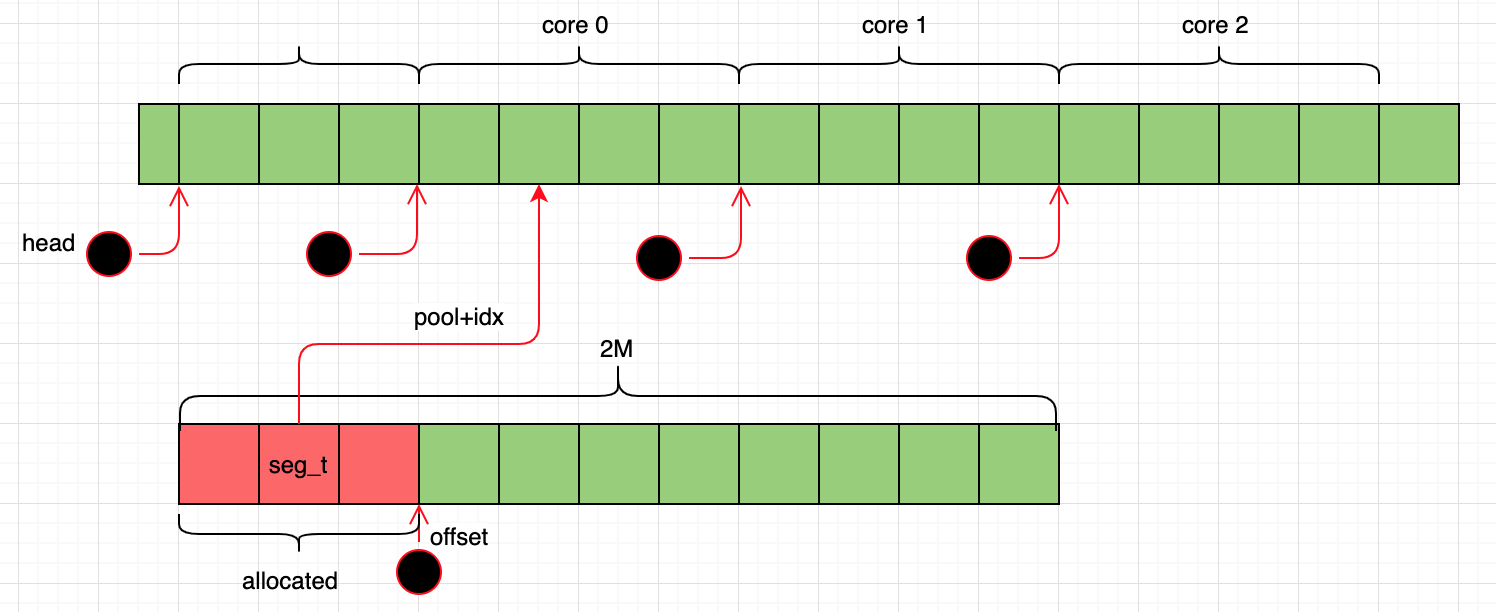
\includegraphics[width=10cm]{../imgs/buffer-t.png}
\end{center}

每个内存区域的\hl{第一个hugepage用来保存该区域的元数据信息},可供分配的是后面的hugepages。
在元数据信息中加上buddy,可用来支持buddy算法。

buffer的每个seg都包含有虚拟地址和物理地址。

\subsection{Memory Pool}

\begin{center}
    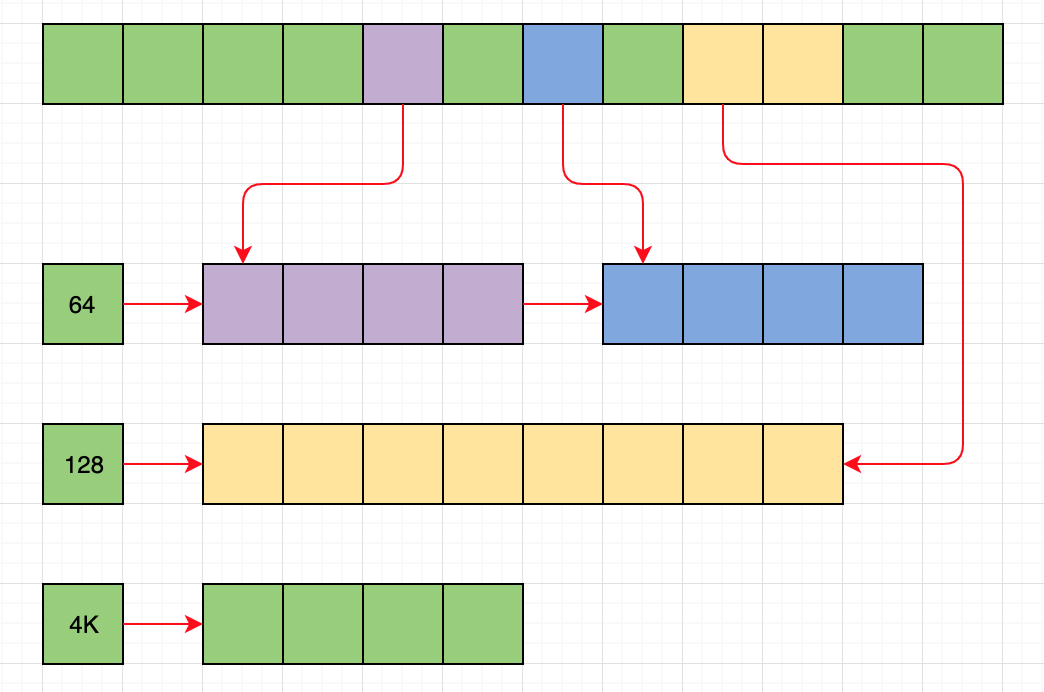
\includegraphics[width=10cm]{../imgs/memory-pool.png}
\end{center}

直接从hugepage申请内存,从hugepage申请一个hugepage,用于小对象。pool管理多个size的小对象队列。
根据要malloc的size,定位到队列。

free时按指针查找属于哪个hugepage。每个hugepge对应起始地址和结束地址以及所在队列的标识。
这样可以保留malloc和free的语法和语义。

hugepage层只需要提供分配单个hugepage的接口,一个队列可以由一个或多个hugepage构成。

或者,memory pool按4k进行组织,同样采用buddy算法。在其上实现ring等。

\hl{每layer都要动态化,包括增和减}。

\subsection{NVMe}

NVMe为什么需要物理地址?

direct io需要512对齐。

\subsection{RDMA}

每个连接$1024*512$内存。

\subsection{IO}

\begin{center}
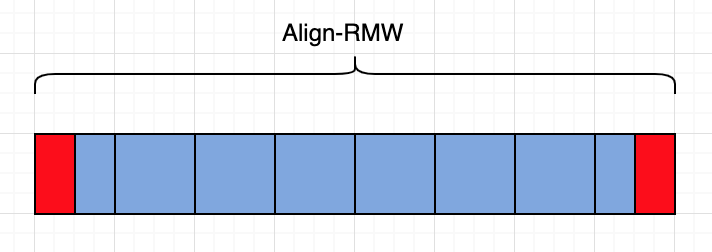
\includegraphics[width=10cm]{../imgs/io-align.png}
\end{center}

首尾页对齐

buffer\_t包含一个seg时,方便处理。如果有多个seg,是否需要分配连续的大块内存。

\hl{SPDK的大IO问题}:NVMe需要物理内存,并且一次io物理内存是连续的。
malloc的内存,不容易找到物理内存。
2M的hugepage虽然能获取虚拟地址连续的4M地址空间,但底层物理内存未必连续。
用1G的hugepage更容易管理。

GFM的机制是什么?barrier去解决RMW、chunk恢复等问题?


\part{生态系统}

\chapter{CEPH}

%\include{sheepdog}
%\include{openvstorage}
%\include{VSAN}

\part{理论基础}

\chapter{分布式系统}

Lich涉及许多底层理论和系统,包括并行计算和分布式系统,操作系统,文件系统,数据库系统,网络,还包括相应的底层硬件架构。
需要对数据结构和算法,有良好基础。所以,对基本问题和理论,要有清晰和深入的掌握,才能“运用之妙,存乎一心”。

存储中一些重要的问题,可以借助AI的力量去解决。智能存储,不仅仅是口号,更是技术进步的必要趋势。

按道法术器组织结构,写成大文章。

常用优化原则:
\begin{itemize}
    \item 局部性
    \item 并行
    \item 聚合,批处理
    \item 延迟
\end{itemize}

\chapter{Parallel Computing}

pattern
\begin{itemize}
    \item pipeline
    \item fork and join
\end{itemize}

\chapter{Design Pattern}

\begin{itemize}
    \item journalling
    \item update many, commit one
    \item double check
    \item double/multi buffer
    \item half sync, half async
\end{itemize}

\chapter{FlowChart}

% 流程图定义基本形状
\tikzstyle{startstop} = [rectangle, rounded corners, minimum width=3cm, minimum height=1cm,text centered, draw=black, fill=red!30]
\tikzstyle{io} = [trapezium, trapezium left angle=70, trapezium right angle=110, minimum width=3cm, minimum height=1cm, text centered, draw=black, fill=blue!30]
\tikzstyle{process} = [rectangle, minimum width=3cm, minimum height=1cm, text centered, draw=black, fill=orange!30]
\tikzstyle{decision} = [diamond, minimum width=3cm, minimum height=1cm, text centered, draw=black, fill=green!30]
\tikzstyle{arrow} = [thick,->,>=stealth]

\begin{tikzpicture}[node distance=2cm]
%定义流程图具体形状
\node (start) [startstop] {Start};
\node (in1) [io, below of=start] {Input};
\node (pro1) [process, below of=in1] {Process 1};
\node (dec1) [decision, below of=pro1, yshift=-0.5cm] {Decision 1};
\node (pro2a) [process, below of=dec1, yshift=-0.5cm] {Process 2a};
\node (pro2b) [process, right of=dec1, xshift=2cm] {Process 2b};
\node (out1) [io, below of=pro2a] {Output};
\node (stop) [startstop, below of=out1] {Stop};

%连接具体形状
\draw [arrow](start) -- (in1);
\draw [arrow](in1) -- (pro1);
\draw [arrow](pro1) -- (dec1);
\draw [arrow](dec1) -- (pro2a);
\draw [arrow](dec1) -- (pro2b);
\draw [arrow](dec1) -- node[anchor=east] {yes} (pro2a);
\draw [arrow](dec1) -- node[anchor=south] {no} (pro2b);
\draw [arrow](pro2b) |- (pro1);
\draw [arrow](pro2a) -- (out1);
\draw [arrow](out1) -- (stop);
\end{tikzpicture}

%作者:红伞菌
%链接:https://www.zhihu.com/question/20854046/answer/16400909
%来源:知乎
%著作权归作者所有。商业转载请联系作者获得授权,非商业转载请注明出处。
%作者:红伞菌
%链接:https://www.zhihu.com/question/20854046/answer/16400909
%来源:知乎
%著作权归作者所有。商业转载请联系作者获得授权,非商业转载请注明出处。

% Defines a `datastore' shape for use in DFDs.  This inherits from a
% rectangle and only draws two horizontal lines.
\makeatletter
\pgfdeclareshape{datastore}{
  \inheritsavedanchors[from=rectangle]
  \inheritanchorborder[from=rectangle]
  \inheritanchor[from=rectangle]{center}
  \inheritanchor[from=rectangle]{base}
  \inheritanchor[from=rectangle]{north}
  \inheritanchor[from=rectangle]{north east}
  \inheritanchor[from=rectangle]{east}
  \inheritanchor[from=rectangle]{south east}
  \inheritanchor[from=rectangle]{south}
  \inheritanchor[from=rectangle]{south west}
  \inheritanchor[from=rectangle]{west}
  \inheritanchor[from=rectangle]{north west}
  \backgroundpath{
    %  store lower right in xa/ya and upper right in xb/yb
    \southwest \pgf@xa=\pgf@x \pgf@ya=\pgf@y
    \northeast \pgf@xb=\pgf@x \pgf@yb=\pgf@y
    \pgfpathmoveto{\pgfpoint{\pgf@xa}{\pgf@ya}}
    \pgfpathlineto{\pgfpoint{\pgf@xb}{\pgf@ya}}
    \pgfpathmoveto{\pgfpoint{\pgf@xa}{\pgf@yb}}
    \pgfpathlineto{\pgfpoint{\pgf@xb}{\pgf@yb}}
 }
}
\makeatother
\begin{center}
\begin{tikzpicture}[
  font=\sffamily,
  every matrix/.style={ampersand replacement=\&,column sep=2cm,row sep=2cm},
  source/.style={draw,thick,rounded corners,fill=yellow!20,inner sep=.3cm},
  process/.style={draw,thick,circle,fill=blue!20},
  sink/.style={source,fill=green!20},
  datastore/.style={draw,very thick,shape=datastore,inner sep=.3cm},
  dots/.style={gray,scale=2},
  to/.style={->,>=stealth',shorten >=1pt,semithick,font=\sffamily\footnotesize},
  every node/.style={align=center}]

  % Position the nodes using a matrix layout
  \matrix{
    \node[source] (hisparcbox) {electronics};
      \& \node[process] (daq) {DAQ}; \& \\

    \& \node[datastore] (buffer) {buffer}; \& \\

    \node[datastore] (storage) {storage};
      \& \node[process] (monitor) {monitor};
      \& \node[sink] (datastore) {datastore}; \\
  };

  % Draw the arrows between the nodes and label them.
  \draw[to] (hisparcbox) -- node[midway,above] {raw events}
      node[midway,below] {level 0} (daq);
  \draw[to] (daq) -- node[midway,right] {raw event data\\level 1} (buffer);
  \draw[to] (buffer) --
      node[midway,right] {raw event data\\level 1} (monitor);
  \draw[to] (monitor) to[bend right=50] node[midway,above] {events}
      node[midway,below] {level 1} (storage);
  \draw[to] (storage) to[bend right=50] node[midway,above] {events}
      node[midway,below] {level 1} (monitor);
  \draw[to] (monitor) -- node[midway,above] {events}
      node[midway,below] {level 1} (datastore);
\end{tikzpicture}
\end{center}

\begin{figure}[htb]
\centering
%定义形状样式
\tikzstyle{startstop} = [rectangle, rounded corners, minimum width = 3cm, minimum height = 0.7cm, text centered, draw = black]
\tikzstyle{startstop2} = [rectangle, rounded corners, minimum width = 13cm, minimum height = 0.7cm, text centered, draw = black]
\tikzstyle{io} = [trapezium, trapezium left angle = 30, trapezium right angle = 150, minimum width = 3cm, text centered, draw = black, fill = white]
\tikzstyle{io2} = [trapezium, trapezium left angle = 30, trapezium right angle = 150, minimum width = 2.5cm, draw = black, fill = white]
\tikzstyle{io3} = [trapezium, trapezium left angle = 30, trapezium right angle = 150, minimum width = 2cm, draw = black, fill = white]
\tikzstyle{process} = [rectangle, minimum width = 3cm, minimum height = 1cm, text centered, draw = black]
\tikzstyle{decision} = [diamond, minimum width = 3cm, minimum height = 1cm, text centered, draw = black]
\tikzstyle{arrow} = [thick, -, >= stealth]
\tikzstyle{arrow2} = [thick, ->, >= stealth]

\begin{tikzpicture}[node distance = 1.5cm]
% 定义流程图具体形状
\coordinate[label = left:{\small 输入图像}](A) at(-1.5, 0);
\node(in1) [io] {};
\node(pro1) [startstop, below of = in1] {\small 线性滤波};

\node(in2 - 2)[io3, below of = pro1, yshift = -0.6cm]{};
\node(in3 - 2)[io3, left of = in2 - 2, xshift = -2.5cm]{};
\node(in4 - 2)[io3, right of = in2 - 2, xshift = 2.5cm]{};

\node(in2 - 1)[io2, below of = pro1, yshift = -0.3cm]{};
\node(in3 - 1)[io2, left of = in2 - 1, xshift = -2.5cm]{};
\node(in4 - 1)[io2, right of = in2 - 1, xshift = 2.5cm]{};

\node(in2) [io, below of = pro1] {\small 颜色};
\node(in3)[io, left of = in2, xshift = -2.5cm]{\small 亮度};
\node(in4)[io, right of = in2, xshift = 2.5cm]{\small 方向};

\node(in5)[startstop2, below of = in2 - 2]{\small Center - Surround差异计算及归一化};

\node(in6 - 2)[io3, below of = in5, yshift = -0.6cm]{};
\node(in7 - 2)[io3, left of = in6 - 2, xshift = -2.5cm]{};
\node(in8 - 2)[io3, right of = in6 - 2, xshift = 2.5cm]{};

\node(in6 - 1)[io2, below of = in5, yshift = -0.3cm]{};
\node(in7 - 1)[io2, left of = in6 - 1, xshift = -2.5cm]{};
\node(in8 - 1)[io2, right of = in6 - 1, xshift = 2.5cm]{};

\node(in6) [io, below of = in5] {};
\node(in7)[io, left of = in6, xshift = -2.5cm]{};
\node(in8)[io, right of = in6, xshift = 2.5cm]{};

\coordinate[label = left:{\small 特征图}](B) at(-1, -6.2);
\coordinate[label = left:{\small (12张)}](C) at(-1.5, -7.5);
\coordinate[label = left:{\small (6张)}](D) at(2.7, -7.5);
\coordinate[label = left:{\small (24张)}](E) at(6.7, -7.5);

\node(in9)[startstop2, below of = in6 - 2]{ \small 跨尺度合并及归一化 };

\node(in10) [io, below of = in9] {};
\node(in11)[io, left of = in10, xshift = -2.5cm]{};
\node(in12)[io, right of = in10, xshift = 2.5cm]{};

\coordinate[label = left:{\small 醒目图}](F) at(-1, -9.5);
\node(in13) [startstop, below of = in10] {\small 线性组合};
\node(in14) [io, below of = in13] {};
\coordinate[label = left:{\small 显著图}](G) at(-1, -13);

\node(in15) [startstop, below of = in14] {\small 赢者取全};
\coordinate[label = left:{\small 显著位置}]() at(1, -16.1);
\coordinate[label = left:{\small 反馈抑制}]() at(4.5, -14.7);

%连线
\draw[arrow](pro1) -- (in1);
\draw[arrow](pro1) -- (in2);
\draw[arrow](pro1) -- (in3);
\draw[arrow](pro1) -- (in4);
\draw[arrow](0, -4.75) -- (in2 - 2);
\draw[arrow](-4, -4.75) -- (in3 - 2);
\draw[arrow](4, -4.75) -- (in4 - 2);
\draw[arrow](0, -5.45) -- (in6);
\draw[arrow](-4, -5.45) -- (in7);
\draw[arrow](4, -5.45) -- (in8);
\draw[arrow](0, -8.35) -- (in6 - 2);
\draw[arrow](-4, -8.35) -- (in7 - 2);
\draw[arrow](4, -8.35) -- (in8 - 2);
\draw[arrow](0, -9.05) -- (in10);
\draw[arrow](-4, -9.05) -- (in11);
\draw[arrow](4, -9.05) -- (in12);
\draw[arrow](in13) -- (in10);
\draw[arrow](in13) -- (in11);
\draw[arrow](in13) -- (in12);
\draw[arrow](in13) -- (in14);
\draw[arrow](in14) -- (in15);
\draw[arrow](in15) -- (0, -15.8);
\draw[arrow](0, -15.4) -- (2.5, -15.4);
\draw[arrow](2.5, -14) -- (2.5, -15.4);
\draw[arrow2](2.5, -14) -- (0, -14);
\end{tikzpicture}
\caption{IT算法流程\cite{Itti}}
\end{figure}

% 设置颜色代号
\colorlet{lcfree}{green}
\colorlet{lcnorm}{blue}
\colorlet{lccong}{red}
% -------------------------------------------------
% 设置调试标志层
\pgfdeclarelayer{marx}
\pgfsetlayers{main,marx}
% 标记坐标点的宏定义。交换下面两个定义关闭。
\providecommand{\cmark}[2][]{%
  \begin{pgfonlayer}{marx}
    \node [nmark] at (c#2#1) {#2};
  \end{pgfonlayer}{marx}
  } 
\providecommand{\cmark}[2][]{\relax} 
% -------------------------------------------------
% 开始绘图
\begin{figure}[h]
\centering
\scalebox{.8}{                  %设置缩放	
\begin{tikzpicture}[
    >=triangle 60,              % 箭头的形状
    start chain=going below,    % 从上往下的流程
    node distance=6mm and 60mm, % 全局间距设置
    every join/.style={norm},   % 连接线的默认设置
    ]
% ------------------------------------------------- 
% 节点的样式定义 
% <on chain> 和 <on grid> 可以减少手动调整节点位置的麻烦
\tikzset{
  base/.style={draw, on chain, on grid, align=center, minimum height=4ex},
  proc/.style={base, rectangle, text width=8em},
  test/.style={base, diamond, aspect=2, text width=5em},
  term/.style={proc, rounded corners},
  % coord 用来表示连接线的转折点
  coord/.style={coordinate, on chain, on grid, node distance=6mm and 25mm},
  % nmark 用来表示调试标志
  nmark/.style={draw, cyan, circle, font={\sffamily\bfseries}},
  % -------------------------------------------------
  % 不同的连接线样式
  norm/.style={->, draw, lcnorm},
  free/.style={->, draw, lcfree},
  cong/.style={->, draw, lccong},
  it/.style={font={\small\itshape}}
}
% -------------------------------------------------
% 先放节点
\node [term, densely dotted,fill=lccong!25, it] (p0) {输入};
% 用 join 表示和上一个节点相连 
\node [proc, join]	{使用非线性最小二乘法得到 $X_0$};
\node [proc, join]	{记录 $X=X_0, f=f(X_0)$};
\node [test, join] (t1)	{$T>T_E$?};
\node [proc] (p1)		{$step=0$};
\node [test, join] (t2)	{$step<count$?};
\node [proc] (p2)		{得到新状态$P_N=P+scale\times rand$,计算目标函数差$\Delta f$};
\node [test, join] (t3)	{$F_{Accept}<rand$?};
\node [proc] (p3)		{记录新状态 $X=X_N,f=f(X_N)$};

\node [proc, left=of t1] (p4)	{$T=T\times a,scale=scale\times b$};
\node [term, densely dotted, right=of t1,fill=lcfree!25](p5)	{输出};
\node [proc, right=of t3](p6)	{$step++$};

\node [coord, left=of t2] (c1)  {}; 
\node [coord, right=of t2] (c2)  {}; 
\node [coord, right=of p3] (c3)  {}; 
%先画南北方向的连接线,先画线再画两端的标志和箭头
\path (t1.south) to node [near start, xshift=1em] {$y$} (p1);
  \draw [*->,lcnorm] (t1.south) -- (p1);
\path (t2.south) to node [near start, xshift=1em] {$y$} (p2);
  \draw [*->,lcnorm] (t2.south) -- (p2);
\path (t3.south) to node [near start, xshift=1em] {$y$} (p3);
  \draw [*->,lcnorm] (t3.south) -- (p3);
%接着画东西方向的连接线,方法同上
\path (t1.east) to node [near start, yshift=1em]  {$n$}(p5);
  \draw [o->,lcnorm] (t1.east) -- (p5);
  \draw [->,lcnorm] (p4.east) -- (t1);
\path (t3.east) to node [near start, yshift=1em]  {$n$}(p6);
  \draw [o->,lcnorm] (t3.east) -- (p6);
\path (t2.west) to node [near start, yshift=1em]  {$n$}(c1);
  \draw [o->,lcnorm] (t2.west) -- (c1) -| (p4);
  \draw [->,lcnorm] (p3.east) -- (c3) -| (p6.south);
  \draw [<-,lcnorm] (t2.east) -- (c2) -| (p6.north);
\end{tikzpicture}
}
\label{fig:algorithm}
\end{figure}

\tikzstyle{every node}=[draw=black,thick,anchor=west]
\tikzstyle{selected}=[draw=red,fill=red!30]
\tikzstyle{optional}=[dashed,fill=gray!50]
\begin{tikzpicture}[%
  grow via three points={one child at (0.5,-0.7) and
  two children at (0.5,-0.7) and (0.5,-1.4)},
  edge from parent path={(\tikzparentnode.south) |- (\tikzchildnode.west)}]
  \node {texmf}
    child { node {doc}}
    child { node {fonts}}
    child { node {source}}
    child { node [selected] {tex}
      child { node {generic}}
      child { node [optional] {latex}}
      child { node {plain}}
    }
    child [missing] {}
    child [missing] {}
    child [missing] {}
    child {node {texdoc}};
\end{tikzpicture}

\begin{tikzpicture}[sibling distance=10em,
    every node/.style = {shape=rectangle, rounded corners,
        draw, align=center,
        top color=white, bottom color=blue!20}]]
        \node {root}
        child { node {snap1} }
        child { node {snap2}
            child { node {snap3}
                child { node {snap4} }
                child { node {snap5} }
                child { node {snap6} } }
            child { node {snap7} } };
\end{tikzpicture}

\begin{tikzpicture}
  \begin{scope}[blend group = soft light]
    \fill[red!30!white]   ( 90:1.2) circle (2);
    \fill[green!30!white] (210:1.2) circle (2);
    \fill[blue!30!white]  (330:1.2) circle (2);
  \end{scope}
  \node at ( 90:2)    {Typography};
  \node at ( 210:2)   {Design};
  \node at ( 330:2)   {Coding};
  \node [font=\Large] {\LaTeX};
\end{tikzpicture}

% Drawing part, node distance is 1.5 cm and every node
% is prefilled with white background
\begin{tikzpicture}[node distance=1.5cm,
    every node/.style={fill=white, font=\sffamily}, align=center]
  % Specification of nodes (position, etc.)
  \node (start)             [activityStarts]              {Activity starts};
  \node (onCreateBlock)     [process, below of=start]          {onCreate()};
  \node (onStartBlock)      [process, below of=onCreateBlock]   {onStart()};
  \node (onResumeBlock)     [process, below of=onStartBlock]   {onResume()};
  \node (activityRuns)      [activityRuns, below of=onResumeBlock]
                                                      {Activity is running};
  \node (onPauseBlock)      [process, below of=activityRuns, yshift=-1cm]
                                                                {onPause()};
  \node (onStopBlock)       [process, below of=onPauseBlock, yshift=-1cm]
                                                                 {onStop()};
  \node (onDestroyBlock)    [process, below of=onStopBlock, yshift=-1cm] 
                                                              {onDestroy()};
  \node (onRestartBlock)    [process, right of=onStartBlock, xshift=4cm]
                                                              {onRestart()};
  \node (ActivityEnds)      [startstop, left of=activityRuns, xshift=-4cm]
                                                        {Process is killed};
  \node (ActivityDestroyed) [startstop, below of=onDestroyBlock]
                                                    {Activity is shut down};     
  % Specification of lines between nodes specified above
  % with aditional nodes for description 
  \draw[->]             (start) -- (onCreateBlock);
  \draw[->]     (onCreateBlock) -- (onStartBlock);
  \draw[->]      (onStartBlock) -- (onResumeBlock);
  \draw[->]     (onResumeBlock) -- (activityRuns);
  \draw[->]      (activityRuns) -- node[text width=4cm]
                                   {Another activity comes in
                                    front of the activity} (onPauseBlock);
  \draw[->]      (onPauseBlock) -- node {The activity is no longer visible}
                                   (onStopBlock);
  \draw[->]       (onStopBlock) -- node {The activity is shut down by
                                   user or system} (onDestroyBlock);
  \draw[->]    (onRestartBlock) -- (onStartBlock);
  \draw[->]       (onStopBlock) -| node[yshift=1.25cm, text width=3cm]
                                   {The activity comes to the foreground}
                                   (onRestartBlock);
  \draw[->]    (onDestroyBlock) -- (ActivityDestroyed);
  \draw[->]      (onPauseBlock) -| node(priorityXMemory)
                                   {higher priority $\rightarrow$ more memory}
                                   (ActivityEnds);
  \draw           (onStopBlock) -| (priorityXMemory);
  \draw[->]     (ActivityEnds)  |- node [yshift=-2cm, text width=3.1cm]
                                    {User navigates back to the activity}
                                    (onCreateBlock);
  \draw[->] (onPauseBlock.east) -- ++(2.6,0) -- ++(0,2) -- ++(0,2) --                
     node[xshift=1.2cm,yshift=-1.5cm, text width=2.5cm]
     {The activity comes to the foreground}(onResumeBlock.east);
\end{tikzpicture}


\end{document}
